\documentclass[a4paper]{article}

%deixa no padr?o brasileiro, traduzindo as se??es, possibilitando caracteres e hifen
\usepackage[brazilian]{babel}
\usepackage[utf8]{inputenc}
\usepackage[T1]{fontenc}

%estilo de header
\pagestyle{headings}

%pacote para inserir imagem
\usepackage{graphicx}

%t?tulo
\title{Ferramentas didáticas de análise léxica}
\author{Gustavo Scaloni Vendramini    \\ 
        Guilherme José Henrique       \\
        Sean Carlisto de Alvarenga    \\
        Vinícius Fernandes de Jesus}
\date{\today}

%pacote que coloca links no table of contents e monta o índice lateral, de acordo com as se??es do documento.
\usepackage[pdftex]{hyperref}

%documento em s?
\begin{document}
\maketitle
\pagebreak
\maketitle
\tableofcontents
%!TEX root = ../relatorio.tex
\section{resumo} % (fold)
\label{sec:resumo}

% section resumo (end)
%!TEX root = ../artigo.tex
\section{sintelo} % (fold)
\label{sec:sintelo}
A ferramenta sintelo é uma ferramenta didática para o ensino de compiladores. A mesma foi criada por Karina Kieling Dos Santos e Philipe Marcon Dos Reis, no ano de 2008 como Trabalho de Conclusão de Curso pela Universidade
do Sul de Santa Catarina e foi publicada em \cite{sintelo}. 

Embora a ferramenta em questão possua mais funcionalidades, esse trabalho se limitou a parte de análise léxica, permanecendo em seu escopo.

Para que possamos realizar a análise léxica, primeiramente devemos informar ao sintelo os tokens de nossa linguagem, através de expressões regulares. Essas expressões regulares devem ser informadas na ``caixa'' chamada léxico, conforme ilustrado na figura~\ref{sintelo-inicial}.

\begin{figure}[ht!]
	\centering
	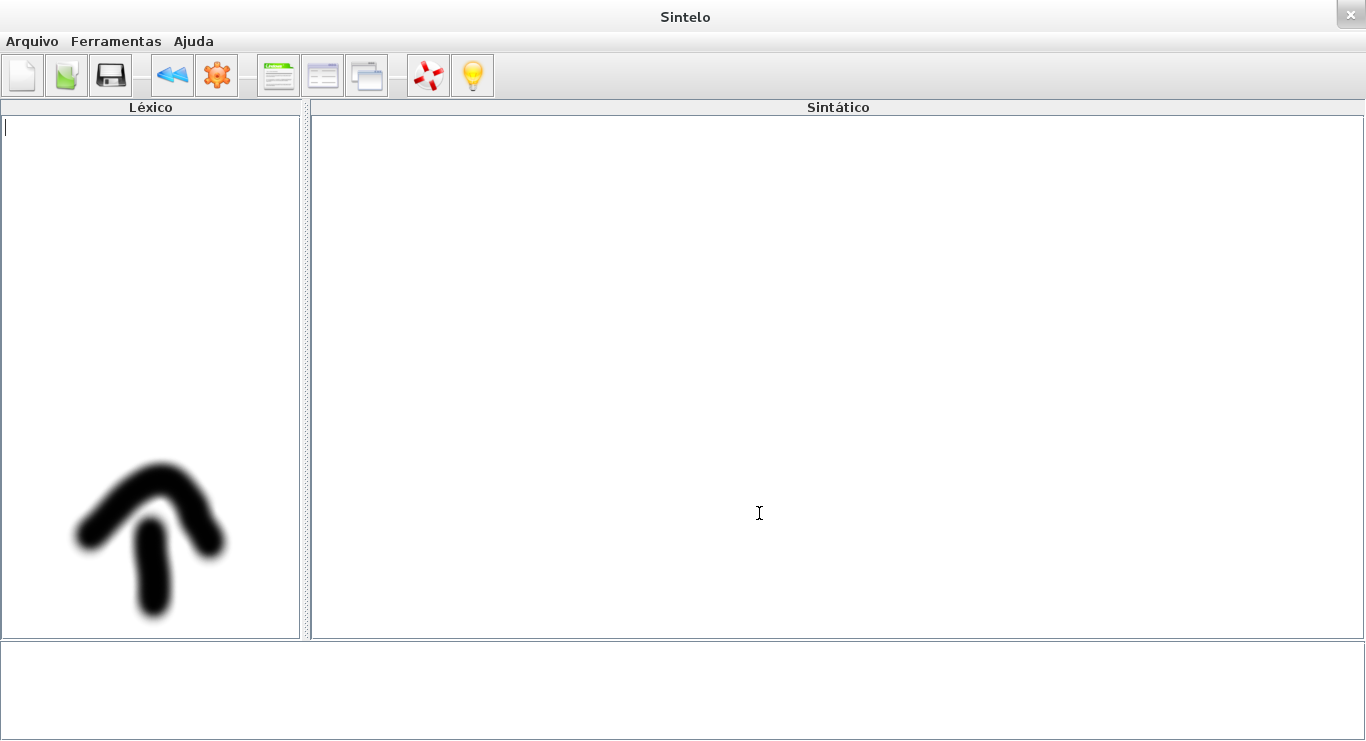
\includegraphics[scale=0.28]{imgs/sintelo-inicial-ed}
	\caption{Tela inicial do sintelo}
	\label{sintelo-inicial}
\end{figure}

A notação utilizada para representar as expressões regulares são descritas em \cite{sintelo} ou no manual da ferramenta, que pode ser acessado através do menu ``Ajuda'', item ``Manual'' e seção ``Especificações Léxicas''. Desta forma este artigo não explicará a notação.

Para exibir a análise léxica, o exemplo de operações aritméticas de \cite{Sebesta201201} será adaptado. Esse exemplo reconhece operações aritméticas que podem conter números (inteiros e/ou reias), identificadores (variáveis), operações binárias e também parêntesis; ignorando espaços em branco, quebra de linha e tabulação.

A seguir, a especificação dos tokens que deve ser passada para o sintelo:
\begin{verbatim}
ID:[a-zA-Z_][_a-zA-Z0-9]*
INT:[0-9]+
REAL:([0-9]\.[0-9]+) | ([0-9]+\.[0-9])
"("
")"
binop:"+" | \- | \*|"/"
:[\s\n\t]+
\end{verbatim}


% section sintelo (end)
\section{Verto} % (fold)
\label{sec:verto}

O Compilador didático Verto é uma aplicação para o suporte pedagógico nas disciplinas de compiladores.
Foi desenvolvido no Centro universitário Feevale para auxiliar os professores na disciplina de compiladores.
e foi lançado sob a licença GPL (GNU General Public
License). Com esse ambiente, os autores proporcionam aos estudantes um projeto 
educativo e bem documentado para sua utilização em seu aprendizado \cite{verto}.

A linguagem fonte para esse compilador foi projetada para ser uma espécie de
português procedural com uma sintaxe parecida com a da linguagem C.
A linguagem objeto escolhida foi a linguagem César \cite{cesar}, uma
linguagem de máquina hipotética implementada na UFRGS.

O software Verto traz o compilador Verto, um editor, parâmetros para o compilador,
um manual de ajuda para os usuários e painéis com informações dos passos 
da compilação do código-fonte inserido no editor do Verto,
como os tokens identificados pelo analisador léxico e as regras reconhecidas da gramática.
Nosso artigo apresenta apenas os aspectos léxicos desse software.

Esse trabalho se propõe a mostrar as funcionalidades e aplicações do compilador Verto 
na parte de análise léxica.
Além disso, os autores desse trabalho ampliaram o escopo do analisador léxico do Verto 
ao estendê-lo para a inserção de novos analisadores.
Como exemplo, foi implementado o \emph{parser} 
que realiza o reconhecimento dos tokens das linguagens Java e Lisp.


\begin{figure}[ht!]
	\centering
	
\includegraphics[scale=0.7]{imgs/Verto.png}
	\caption{Logo do software Verto}
	\label{verto-inicial}
\end{figure}

\subsection{Exemplo} % (fold)
\label{sub:exemplo-verto}

O software Verto traz um editor que destaca em azul as palavras-chaves de acordo com a linguagem selecionada.
A Figure \ref{editor-azul} mostra esse comportamento.
\begin{figure}[ht!]
	\centering
	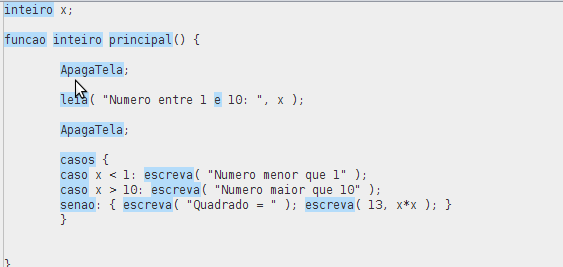
\includegraphics[scale=0.7]{imgs/editor-azul.png}
	\caption{Editor com destaque de palavras}
	\label{editor-azul}
\end{figure}


Depois de implementado seu programa, o próximo passo seria escolher a opção Compilar no menu ou
digitar as teclas de atalho Ctrl+K.
Um erro encontrado é que quando o destaque de palavras-chave está habilitado essas teclas de atalho não funcionam,
obrigando o usuário a compilar a partir do menu.
A figura \ref{opcao-compilar} ilustra isso.
\begin{figure}[ht!]
	\centering
	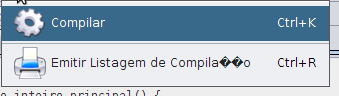
\includegraphics[scale=0.7]{imgs/compilar-opcao.png}
	\caption{Opção de compilar tanto no mouse quanto em atalhos do teclado}
	\label{opcao-compilar}
\end{figure}


Após a compilação, o Verto traz a tabela com as informações particulares que cada fase do compilador gerou.
Na Figura \ref{tabela-tokens} estão alguns tokens identificados com a linguagem do Verto com os seus respectivos lexemas.
Um defeito encontrado é que o painel que se encontra essas tabelas não permite o seu redimensionamento.
\begin{figure}[ht!]
	\centering
	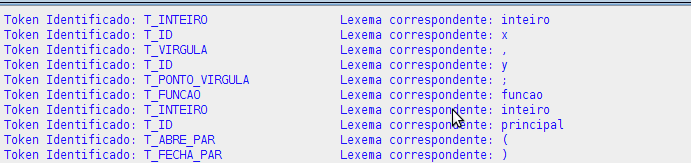
\includegraphics[scale=0.7]{imgs/tabela-tokens.png}
	\caption{Tabela de tokens gerada pelo analisado léxico}
	\label{tabela-tokens}
\end{figure}


\subsection{Extensão do Verto}
Uma das contribuições que nosso trabalho traz é um \emph{framework} que permite a extensão da arquitetura do Verto.
Como o escopo do nosso trabalho é a etapa léxica, a implementação se restringiu a esta parte.
que permite a construção de nossos compiladores.
Isso, no âmbito pedagógico, pode proporcionar uma nova perspectiva no aprendizado do aluno,
ja que, em cursos de compiladores, geralmente o ensino se limita a uma visão mais simplista e de alto nível.
Com essa abordagem, o aluno ajudaria a programar a construção de um compilador, estendendo os componentes do \emph{framework}.

A ideia principal desse \emph{framework} é quebrar o algoritmo de cada fase do compilador
em classes distintas.
As partes do algoritmo que são independentes de linguagem serão implementadas em uma classe pai, 
por exemplo, a classe "Lexico", "Semantico" e "Sintático". 
Depois disso, por meio de métodos abstratos, as partes que são intrínsecas às linguagens, serão implementadas
nos métodos filhos, por exemplo, "LispLexico", "LispSemantico" e "LispSintatico".
Esse projeto foi altamente inspirado no \emph{design pattern Template Method} \cite{gof}.
Por ora, devido ao escopo do projeto, só foi implementada a parte léxica desse \emph{framework}
A Imagem \ref{diagrama-classe}  mostra o exemplo dessa arquitetura para o léxico.
\begin{figure}[ht]
	\centering
	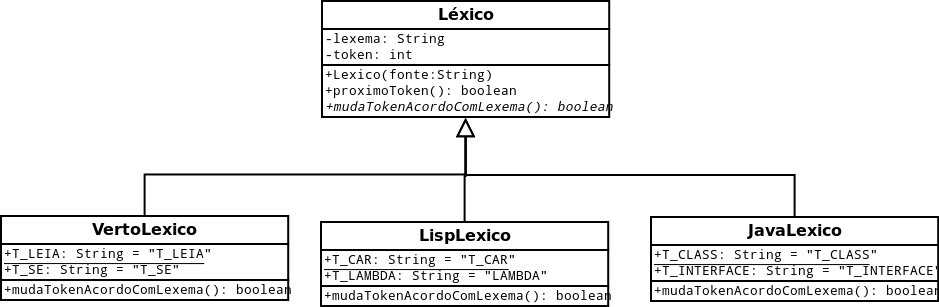
\includegraphics[scale=0.4]{imgs/diagrama-classe.png}
	\caption{Esboço da arquitetura planejada}
	\label{diagrama-classe}
\end{figure}

A escolha da linguagem dentro da interface gráfica será realizada no menu da configuração.
\begin{figure}[ht]
	\centering
	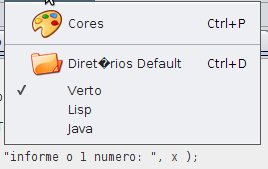
\includegraphics[scale=0.7]{imgs/escolha-linguagem.png}
	\caption{Escolha da linguagem}
	\label{escolha-linguagem}
\end{figure}

As Figuras \ref{lisp-lexico} e \ref{java-lexico} mostram o resultado do léxico para as linguagens Java e Lisp.
Note o destaque das palavras, que são dinâmicos de acordo com a linguagem.

\begin{figure}[ht]
	\centering
	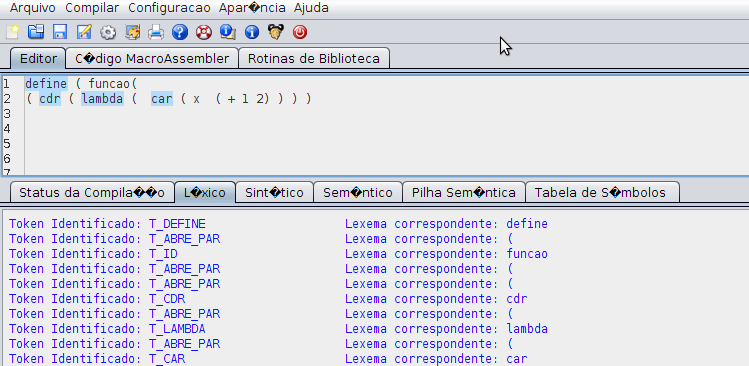
\includegraphics[scale=0.7]{imgs/lisp-lexico.png}
	\caption{Léxico para a linguagem Lisp}
	\label{lisp-lexico}
\end{figure}

\begin{figure}[ht]
	\centering
	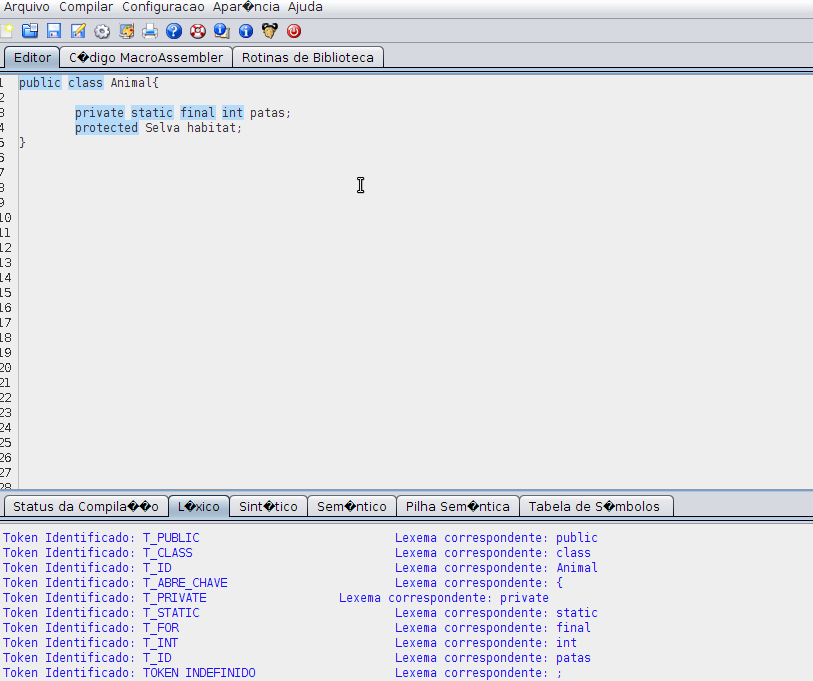
\includegraphics[scale=0.7]{imgs/java-lexico.png}
	\caption{Léxico para a linguagem Java}
	\label{java-lexico}
\end{figure}

http://verto.sourceforge.net/
\subsection{Considerações}
\label{sub:consideracoes-verto}
O compilador educativo Verto é de fácil uso e cumpre bem o seu propósito.
Seus pontos fortes são a leitura de sua linguagem fonte ser em português -
o que pode facilitar para quem é iniciante na programação, a geração de código para
uma máquina hipotética simples e os detalhes dos passos de compilação.
Além disso, uma grande vantagem observada, que a maioria dos compiladores educativos não fornecem
é o fácil acesso ao código-fonte e uma considerável documentação.

Seus pontos fracos são seus pequenos bugs que podem atrapalhar a experiência do usuário e
a realização do processo de compilação em uma única linguagem, o que pode inibir o 
desejo do aluno de se construir um um compilador.

Com essa limitação natural do Verto, foi proposta uma ampliação da
arquitetura do Verto para construção de novos compiladores, utilizando-se de
um projeto de fácil manutenção que possibilitará grande reaproveitamento de código e
facilidade de extensão.

\begin{tabular}{|m{1.6cm}|m{1.5cm}|m{1.5cm}|m{1.5cm}|m{1.5cm}|m{1.8cm}|m{1.5cm}|}  \hline
   Ferramenta & Design da interface com o usuário & Facilidade de uso da ferramenta & Interação com o usuário & Facilidade de aplicação da fundamentação teórica & Capacidade de aplicação das ramificações teóricas & Relação entre uso e aprendizado \\ \hline
C-gen & Bom & Regular & Bom & Ótimo & Ruim & Bom \\ \hline
\end{tabular}





\bibliographystyle{plain} % especifica o estilo como as refer?ncias s?o formatadas
\bibliography{artigo} % especifica o arquivo que cont?m todas as refer?ncias catalogadas, de acordo com a sintaxe de um arquivo .bib.
\end{document}